\documentclass[a4paper,9pt]{article}
\usepackage[a4paper, hmargin={1.5cm,1.5cm}, vmargin={1.5cm,1.5cm}]{geometry}
\usepackage{amsmath}
\usepackage{amsthm}
\usepackage{amsfonts}
\usepackage{color}
\usepackage[final]{graphicx}
\usepackage{subcaption}
\usepackage{wrapfig}
\newtheorem{remark}{Remark}[]
\newtheorem{prop}{Proposition}
\newtheorem{prob}{Problem}
\usepackage{amssymb}
\usepackage{verbatim}
\usepackage{listings}

\newcommand{\R}{\mathbb{R}}
\newcommand{\C}{\mathbb{C}}
\newcommand{\N}{\mathbb{N}}
\newcommand{\Q}{\mathbb{Q}}
\newcommand{\W}{\mathbb{W}}
\newcommand{\Vspace}{\mathbb{V}}
\newcommand{\Hspace}{\mathbb{H}}
\newcommand{\Lspace}{\mathbb{L}}
\newcommand{\Lagr}{\mathcal{L}}


% Title Page
\title{Topics in Computational Science Report \\ Logistic Map and Sensitivity on Initial Condition}
\author{Alifian Mahardhika Maulana}


\begin{document}
\maketitle
\begin{enumerate}
	\item Plot the solution of the following map:
	\begin{equation}\label{eq:1}
	\begin{cases}
	x_{n+1} = ax_n(1-x_n), & n = 1\cdots 100\\
	x_0 = 0.35
	\end{cases}
	\end{equation}
	\begin{enumerate}
		\item a = 0.5
		\item a = 1.5
		\item a = 3.3
		\item a = 4.0
	\end{enumerate}
\end{enumerate}
Below is the graph of the solution from \eqref{eq:1}, plotted using Python Code attached on the next page.
\begin{figure}[h!]
	\centering
	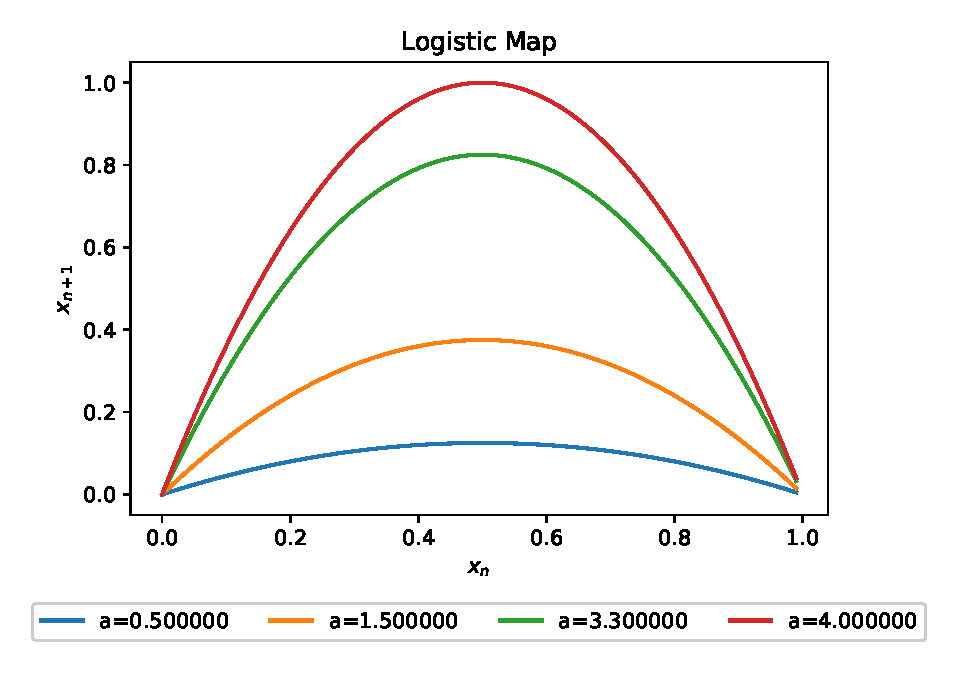
\includegraphics[width=0.5\linewidth]{picture/logisticmap}
	\caption{Logistic Map of various a}
	\label{fig:logisticmap}
\end{figure}
\begin{figure}[h!]
	\centering
	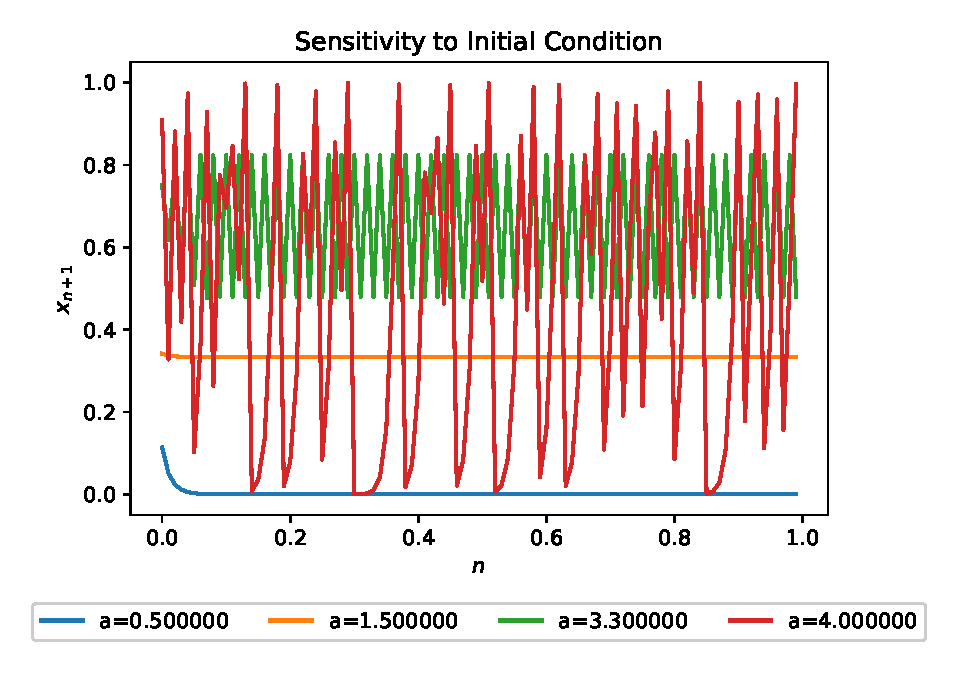
\includegraphics[width=0.5\linewidth]{picture/sensitivity}
	\caption{Sensitivity to Initial Condition Plot}
	\label{fig:sensitivity}
\end{figure}
\newline
\section{Python Code}\label{code}
\lstinputlisting[basicstyle=\ttfamily\scriptsize,language=Python]{logisticmap.py}
\end{document}